
% The \phantomsection command is needed to create a link to a place in the document that is not a
% figure, equation, table, section, subsection, chapter, etc.
% https://tex.stackexchange.com/questions/44088/when-do-i-need-to-invoke-phantomsection
\phantomsection

% Multiple-language document - babel - selectlanguage vs begin/end{otherlanguage}
% https://tex.stackexchange.com/questions/36526/multiple-language-document-babel-selectlanguage-vs-begin-endotherlanguage
\begin{otherlanguage*}{brazil}
% ----------------------------------------------------------
\chapter{Trabalhos Relacionados}\label{cap:trabalhos:relacionados}
% ----------------------------------------------------------

Neste capítulo serão apresentados alguns trabalhos que possuem correlação
com esta monografia, envolvendo os conceitos de \textit{Checkpoint/Restore},
tolerância a falhas e contêineres.

\section{Checkpoint/Restore para contêineres Stateful}

Em \cite{muller2022architecture}, é proposto, como prova de conceito, uma
arquitetura transparente para realizar o \textit{Checkpoint/Restore} de
contêineres \textit{Stateful} utilizando Kubernetes. O foco primário é em
tolerância a falhas com técnicas de \textit{Checkpoint/Restore}, onde se é
abordado a problemática de se ter uma réplica nova do serviço que seja
consistente com o momento atual da falha, não havendo perda de informações
de estado da antiga réplica.

Para o \textit{Checkpoint/Restore} o trabalho propõe a utilização de um
contêiner \textit{sidecar}, o interceptador, que intercepte as requisições
para o contêiner que será feito o \textit{Checkpoint/Restore}. Este contêiner
irá redirecionar as requisições ao contêiner que é feito o \textit{checkpoint}
e também controla o momento do \textit{checkpoint}. Desta forma, é possível
saber quais as requisições que foram processadas pelo contêiner que está sendo
monitorado até o momento do último \textit{checkpoint}, já que a imagem de
\textit{checkpoint} possui metadados salvos no \textit{etcd}. Quando uma nova
réplica deste contêiner for iniciada, teremos a imagem do último
\textit{checkpoint} e o interceptador irá refazer as requisições feitas a
partir do momento do último \textit{checkpoint}, isto permite obter a imagem
mais consistente com o momento da falha do último contêiner que estamos
reinicializando.

Na arquitetura também temos um operador, que é responsável por manter o
estado das aplicações, ele troca informações com o interceptador para remover
contêineres, reiniciá-los ou avisar que eles falharam. Outro ponto da
arquitetura é o administrador de estados, que serve para armazenar e categorizar
as imagens do \textit{checkpoint} com \textit{checksums} e seus metadados no etcd.

Na proposta, se utiliza um monitoramento por \textit{ping} de pacotes para
identificar se um contêiner falhou ou não. No próprio trabalho o autor deixa
claro outros métodos que poderiam ser utilizados, como monitoramento das
informações do contêiner, ou mesmo um indicador de saúde provido pelo contêiner.
A partir do momento de identificação da falha, outro contêiner com a imagem
mais recente de \textit{checkpoint} é criado para substituir o contêiner
falhante. Como o interceptador só confirma uma mensagem quando o contêiner
responde de volta, então, temos certeza de que o interceptador sabe a partir
de qual requisição enviar para recuperar o estado.

Por fim, é apresentada uma prova de conceito realizada em cima do Kubernetes.
A partir da prova de conceito o controlador do StatefulSet foi estendido para
dar suporte ao Operador da arquitetura, e a aplicação a ser monitorada e o
Interceptador foram colocados no mesmo Pod. Conseguiu-se provar ao utilizar o
Kubernetes a possibilidade de utilizar a arquitetura para
\textit{Checkpoint/Restore} para tolerância a falhas. Mas, foram levantados
pontos de melhoria, como, utilização de \textit{checkpointing} ativa, ou seja,
realizando \textit{checkpoint} somente quando uma réplica falhar, para diminuir
o problema de \textit{buffer} em cache dos interceptadores, detecção de falhas
a partir de processos diferentes, como um algoritmo Bizantino, e outros
processos de recuperação pró ativa, como votação para decidir réplicas incorretas.

No contexto do trabalho desenvolvido por nós, este trabalho propõe pontos
importantes para nosso desenvolvimento. Como, por exemplo, como recuperar
exatamente o estado que precisaríamos do nosso serviço. Também é interessante
a abordagem para salvamento de metadados utilizando o etcd que já vem integrado
ao Kubernetes. Nota-se, também, que alguns pontos de melhoria podem ser
priorizados no desenvolvimento de nosso trabalho para ter uma solução mais
abrangente de outras aplicações.

Já em \cite{vayghan2021kubernetes}, os autores propõem uma extensão das
funcionalidades do Kubernetes para contêineres \textit{Stateful} para
prover alta disponibilidade (\textit{High Availability}) à réplicas de um mesmo
microsserviço. Isto implica, que será necessário manter a aplicação disponível
o mais rápido possível depois de ela ter alguma falha.

O trabalho em \cite{vayghan2021kubernetes} aborda uma nova forma de se
utilizar contêineres \textit{Stateful} sem utilizar o StatefulSet do Kubernetes,
mas utilizando o Deployment com um Persistent Volume compartilhado entre todos
os Pods dos quais o Deployment controla. Desta forma, todos os contêineres
compartilham o mesmo armazenamento e tem acesso ao mesmo estado em disco.
Segundo o artigo, nenhum dos dois tipos conseguem suprir necessidades reais de
aplicações de alta disponibilidade, por isso, se faz necessário criar uma
solução que provenha mais velocidade na reinicialização de Pods falhantes.

A solução proposta consiste em ter dois Pods disponíveis provendo o mesmo
serviço em determinado tempo. Um deles é classificado como o ativo, enquanto
o outro é classificado como o "em espera". O Pod que serve requisições é o
ativo, quando este falha, um \textit{controller} criado para isso, State Controller,
copia o estado do Pod falhante para o Pod reserva e cria um novo Service para ele
servir as requisições. Quando o Pod ativo é recuperado, se faz o caminho inverso
para ele voltar a ser o Pod que recebe as requisições. A replicação de estado no
Pod reserva é feito através de um redirecionamento das requisições do Pod ativo,
como o State Controller cria Services separados para os Pods é possível descobrir
o Pod reserva através do nome do Service ao invés de seu IP no \textit{cluster}
graças ao componente de kube-proxy do Kubernetes.

Por fim, são apresentados os experimentos e resultados, tendo em mente que a
alta disponibilidade dos serviços almejada era de 99,999\% anualmente. Os
experimentos consistiram em utilizar um serviço de \textit{streaming} para os
clientes, em que o estado do contêiner consiste no momento que o cliente está
na transmissão de vídeo, utilizando um cluster de oito máquinas e salvando o
estado num Persistent Volume.

As métricas de disponibilidade usadas foram de tempo de reação, o tempo de
reação do Kubernetes para perceber uma falha e iniciar o processo de
recuperação do Pod, o tempo de reparo, tempo a partir da percepção do Kubernetes
até recuperação do Pod, o tempo de recuperação, o tempo a partir da percepção
da falha pelo Kubernetes até a finalização da recuperação e quando o serviço
atinge o estado de pronto, e, por fim, o tempo de indisponibilidade, que
consiste no tempo que o serviço permanece sem disponibilidade, representado
pela soma do tempo de reação com o tempo de recuperação.

Outras métricas obtidas pelo serviço, o State Controller proposto também
foram utilizadas. A métrica de tempo de escala, que é o tempo de percepção
do controlador de estado de um evento de escala até o escalonamento e
disponibilização do serviços escalados para mais ou menos réplicas. A métrica
de tempo de configuração do estado de alta disponibilidade, que é o tempo
para o State Controller agir de acordo com o evento de réplica e configurar
os estados dos Pods para se ter um ativo e outro reserva.

Os experimentos pretendiam responder às cinco perguntas:

\begin{enumerate}
    \item Qual o impacto do State Controller na disponibilidade provida?
    \item Qual o impacto de escalar durante um momento de falha na
    disponibilidade que o State Controller pode prover aos microsserviços
    gerenciados?
    \item Qual é a sobrecarga gerada pelo State Controller no escalonamento?
    \item Qual é o impacto de falhas simultâneas nos Pods ativos no tempo de
    indisponibilidade de cada Pod falhante?
\end{enumerate}

Dos experimentos se obteve respostas:

\begin{enumerate}
    \item Os resultados mostram que é mais rápido para o State Controller
    configurar os estados aos Pods recuperados do que o Kubernetes recuperar
    os serviços. Com uma pequena diferença na velocidade de recuperação entre
    StatefulSets e Deployments, onde o último tem velocidade maior e melhorada
    graças ao State Controller. Apesar do pequeno trabalho a mais que o State
    Controller gera o tempo de recuperação diminui devido ao Pod reserva.
    \item Os resultados mostram que o State Controller gera um atraso no
    escalonamento devido ao tempo que se leva para configurar os estados de
    disponibilidade aos Pods. Como o serviço não consegue realizar as duas
    operações ao mesmo tempo, ocorre um atraso no escalonamento, com maior atraso
    para os escalonamento de menos réplicas.
    \item Os resultados mostram que gera mais trabalho para escalonamento, mesmo
    sem falhas, e que demora mais para as reações de escalonamento ocorrerem
    quando se utiliza o State Controller.
    \item Os resultados mostram que quanto mais tarde um Pod falha mais tarde ele
    será recuperado pelo State Controller, isto ocorre, segundo a autora, pela
    utilização de uma fila \textit{FIFO} para tratamento da recuperação, o que
    gera este problema.
\end{enumerate}

Este trabalho demonstra uma outra forma de abordar o problema de serviços
\textit{Stateful}, ao invés de se salvar o estado em memória, se salva o
estado utilizando os métodos de Persistent Volumes do Kubernetes. Desta
forma, demonstra mais um fator que pode ser interessante observar no
desenvolvimento do nosso trabalho, já que, para algumas aplicações este
estado é interessante. Outro fator importante é a seleção de métricas, que
o artigo aponta algumas métricas importantes para se considerar na avaliação
da adequação da solução.

Já em \cite{schmidttransparent}, temos uma proposta de uma ferramenta para
tolerância a falhas em contêineres \textit{Stateful} no Kubernetes utilizando
\textit{Checkpoint/Restore}. Os autores utilizam a técnica de \textit{Checkpoint}
já disponível no Kubernetes em versão alpha para gerar um ponto de salvamento
do estado do sistema. O Kubernetes utiliza a \textit{runtime} de contêineres
cri-o\cite{cri-o}, que internamente, utiliza o CRIU\cite{criu} para realizar
o \textit{Checkpoint}. Como os autores discutem, este ponto de salvamento
gerado não pode ser utilizado diretamente para executar outro contêiner como
uma imagem.

Para possibilitar a parte do \textit{Restore} os autores desenvolveram uma
aplicação que constrói uma imagem compatível com \textit{Open Container Interface}
que é possível ser utilizada no cri-o. Para o desenvolvimento tanto do sistema
de \textit{Checkpoint} quanto do de \textit{Restore} os autores utilizaram o
conceito de operador do Kubernetes para monitorar o estado dos recursos do 
\textit{cluste} e conciliar para salvar o estado das aplicações monitoradas
através de anotações nos manifestos dos recursos e restaurar quando ao monitorar
se perceber que houve uma falha na aplicação monitorada. Foram integradas outras
funcionalidades ao trabalho, como a possibilidade de integrar diversos nós do
\textit{cluster} para distribuição geográfica e possibilidade de criar formas
diferentes de se verificar se a aplicação falhou, como um recurso de
\textit{liveness}.

Os autores conseguiram prover o serviço, que, como já esperado gera um pouco
de perda de performance nos momentos de realizar o salvamento do estado e da
recuperação. Também é possível ver que durante momentos de salvamento e de
recuperação a latência das aplicações aumenta, pois, durante um
\textit{Checkpoint} a aplicação fica não responsiva, e até a recuperação da
aplicação falhante há outra latência. Entretanto, se verificou que é possível
realizar o \textit{Checkpoint/Restore} de aplicações \textit{Stateful} no
Kubernetes.

\section{Checkpoint/Restore com migração de contêineres Stateful}

Em \cite{oh2018stateful}, os autores desenvolvem uma técnica de
\textit{Checkpoint/Restore} para migração de \textit{clusters} com contêineres
StatefulSet. Como prova de conceito é construída uma aplicação em cima de
Kubernetes e CRIU para realização do \textit{Checkpoint/Restore}. Alguns
motivos levam contêineres em um orquestrador de contêineres ter que ser
movido de um nó para outro, como manutenção do nó atual necessitando de uma
reinicialização, falha do nó atual ou escalonamento e balanceamento de carga
das aplicações do \textit{cluster}. Logo, se um contêiner possui estado,
nestes casos é interessante que a migração dele para um novo nó seja feita
com salvamento do estado passado para reinicializar consistentemente.

Primeiramente, é analisada uma técnica para migração de contêineres
\textit{Stateful} através da utilização de volumes, \textit{Persistent Volumes}
no Kubernetes. Através da análise do autor, se observa que para realizar
uma migração do estado utilizando os volumes, se tem uma complexidade aumentada.
Já que, para salvar o estado em um volume é necessário que a aplicação saiba
realizar esta tarefa, então, não é transparente ao desenvolvedor. Também o
desgaste pelo acesso ao volume que pode ser intermediado por uma API de terceiro,
como no caso de um volume de dados armazenado na EC2 API da Amazon. A partir
desta análise, os autores propõem uma abordagem através da técnica de
\textit{Checkpoint/Restore} com criação de uma imagem com o estado salvo do contêiner.

Para realização da migração eles propõem uma solução que consiste em três
estágios: pré migração, migração e pós-migração. Na pré migração é iniciado
o processo de migração por qualquer motivo, como escalonamento, depois se elege
novos nós para receberem os contêineres do nó antigo, por fim, se criam as
imagens dos contêineres para substituir as antigas. Na migração é realizado
\textit{checkpoint} do contêiner, gerando uma nova imagem, esta imagem é
transmitida para o novo nó através da internet e no novo nó é iniciado um
novo contêiner a partir desta imagem, isto permite que o processo seja
resumido com seu estado passado. Por fim, no estágio de pós migração é
realizada a alocação de recursos antigos, como balanceadores de carga ou
registros \textit{DNS} para o novo contêiner.

Segundo os autores, a solução proposta ainda possui alguns problemas. No
caso de falhas do nó ela não consegue realizar a migração, embora o
\textit{checkpoint} periódico resolveria esta dor, problemas com a internet
para envio da imagem são ignorados no trabalho. Mas, com a proposta se pode obter uma
transparência a nível de aplicação da migração do contêiner, se tem uma
migração leve e ágil, já que, não se usa um volume e, não tem o trabalho
a mais de comunicação com possíveis APIs externas e leitura/escrita de volumes.

Para testar a solução se utilizou um \textit{cluster} de máquinas com um
orquestrador de contêineres e uma aplicação de servidor que incrementava
um contador a cada requisição com o estado salvo em memória. Também se
implementou a solução na linguagem Go, se comunicando com a \textit{engine}
Docker e utilizando o CRIU para realizar o \textit{checkpoint}. Como
observado no trabalho, o tempo de inatividade no processo de migração se
mostra baixo, 576.61ms em média, sendo que o tempo de latência da aplicação
não foi alterado durante a utilização da imagem. Também não houveram
falhas para enviar a imagem de \textit{checkpoint} pela rede para o novo nó.

Embora neste trabalho o conceito abordado de \textit{Checkpoint/Restore}
seja utilizado em um contexto diferente, para migração de aplicações em
\textit{clusters}. Ainda sim, muitos conceitos se relacionam a nosso trabalho.
A utilização de contêineres e aplicações de \textit{Checkpoint/Restore},
diferentemente dos outros trabalhos vistos até o momento, este utiliza uma
outra forma de salvar a imagem de \textit{checkpoint}, que é através do envio
pela rede. Também é abordada a transparência da aplicação, que também é
importante no nosso trabalho, para que não haja adaptação das aplicações
para a solução específica. Por fim, os autores apontam para um ponto
importante que queremos cobrir, que é o caso de tolerância a falhas no caso
de uma falha de nó, como apontado por eles, que por sugestão dos autores
poderia ser resolvida por monitoramento do nó ou mesmo \textit{checkpoints}
periódicos das aplicações com estado.

Já em \cite{tran2022proactive}, os autores propõem uma implementação
para migração de serviços \textit{Stateful} que seja proativa, ou seja,
que perceba antes de uma falha ocorrer no nó e realize a migração para
um novo nó sem que haja a necessidade do nó falhar antes, isto aumenta
a tolerância a falhas e a qualidade de serviço provida. Para isso, os
autores utilizam um algoritmo de \textit{Bidirectional Long Short-Term
Memory} (Bi-LSTM) para predição de falhas. A seleção foi em base do estado
da arte em \textit{Machine Learning}, já que o propósito do artigo é
avaliar a atividade proativa de \textit{Checkpoint/Restore} para
migração dos contêineres. Desta forma, se utilizou o algoritmo para prever
a sobrecarga do uso de CPU como falha.

Para realizar o \textit{Checkpoint/Restore} os autores propõem uma solução
baseada no StatefulSet do Kubernetes, assim como em \cite{vayghan2021kubernetes},
e também um salvamento dos dados em memória através do CRIU, como em
\cite{muller2022architecture}. Desta forma, se tem o estado total da aplicação,
suportando multi \textit{clusters} e \textit{clusters} de nó único.

Para realização das migrações proativas foram criados três aplicações
principais. O \textit{Monitor Framework}, responsável por monitorar as métricas
do \textit{cluster}, como CPU e memória, também lida com o registro de serviços.
O \textit{Fault Prediction Framework}, responsável pelo modelo de predição
de falha, que possui dois processos, o processo \textit{offline}, que realiza
o treinamento com base nos dados recebidos do \textit{Monitor Framework} sobre
a métrica de CPU, e, o processo \textit{online}, que realiza a execução do
modelo com a predição da falha do nó. Por último, temos a funcionalidade
nativa de migração de \textit{clusters}, que é uma modificação do Kubernetes,
componente kubelet, para possibilitar a utilização da predição e da migração
entre dois \textit{clusters}. Podemos ver esta arquitetura demonstrada na
Figura \ref{fig:proactive}.

\begin{figure}[h]
\centering
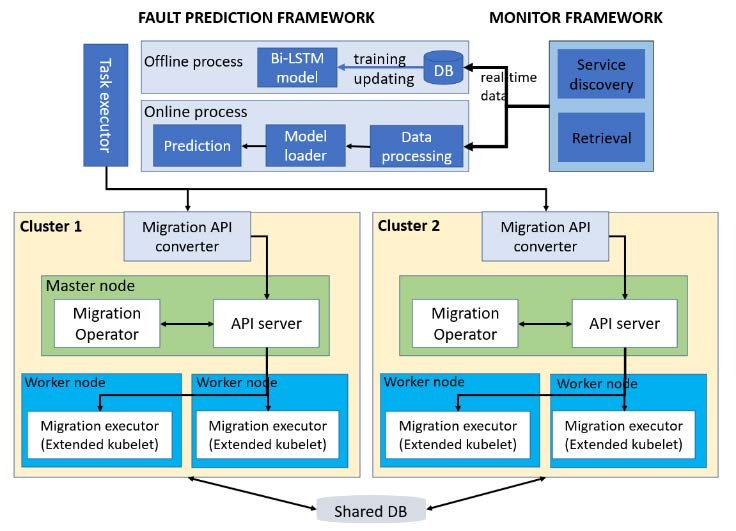
\includegraphics[scale=0.54]{images/proactive-architecture.png}
\caption{Arquitetura de migração proativa de contêineres em \textit{clusters}.}
\label{fig:proactive}
\fonte{\cite{tran2022proactive}}
\end{figure}

Para realizar a migração foi modificado o componente kubelet do Kubernetes e
também a \textit{runtime} de contêineres em utilização pelo Kubernetes para
possibilitar a comunicação com o CRIU para realizar o \textit{Checkpoint/Restore}
dos processos dos contêineres a serem migrados. Desta forma, quando uma migração
é solicitada, primeiro se realiza o \textit{Checkpoint/Restore} de todos os
contêineres no Pod solicitado para migrar, depois se envia a imagem ao novo nó
que ele irá executar. O novo nó utiliza a imagem gerada do \textit{Checkpoint}
para restaurar o estado antigo, só então são excluídos o Pod antigo e
redirecionado o Service ao novo.

Para o processo de migração se utilizou o conceito de Operator do Kubernetes
e \textit{Custom Resource Definitions} (CRDs), que permitem a definição de
novos recursos de API e da criação de novos controladores para monitorar a
API e alcançar o estado desejado dos recursos. Então, em um processo de
migração um novo recurso de migração é adicionado ao Kubernetes e o
controlador da migração deve ser capaz de realizar o Checkpoint do Pod, enviar
para o novo nó, iniciar o Pod no novo nó, eliminar o Pod antigo e reconfigurar
o Service para o novo Pod. Também alteraram a definição da interface de
\textit{runtime} de contêiner do Kubernetes para incluir métodos para realizar
\textit{Checkpoint} e \textit{Restore} com CRIU, desta forma, é possível realizar
as chamadas diretamente pela API do Kubernetes. Por fim, foi utilizado um servidor
de arquivos para armazenar as imagens de \textit{Checkpoint} entre os nós de
migração, desta forma, basta montar o volume nos dois nós e eles estariam
compartilhando as imagens, também se remove a necessidade de envio
por internet da imagem entre os nós e diminui as comunicações.

Para realizar a validação da solução se utilizou quatro \textit{clusters} de
Kubernetes, onde seriam executados aplicações de longo período de inicialização,
como \textit{Mongo-DB} e \textit{Redis}, bem como aplicações de estado baseado na
execução, como FFMPEG, todas executando através de StatefulSets. Para realizar a
migração proativa, o estresse de CPU foi simulado utilizando uma ferramenta que
permite sobrecarregar os nós, \textit{Stress-ng}. Assim, foram verificadas métricas
para resultados, no caso o erro da média da raiz quadrado e o erro de média absoluta
para o modelo de predição e o tempo de recuperação do serviço migrado e a latência
de qualidade de serviço evitada pela migração.

Como resultados foi observado que dos modelos abordados o melhor para a predição
correta através de dois processos é o Bi-LSTM e ele pode ser utilizado para séries
de tempo de diferentes tipos, como CPU, memória e temperatura. Também se observou
que nas aplicações com tempo longo de inicialização houve melhoria do tempo de
recuperação de serviço apenas em redes de alta velocidade, mas, segundo os autores
não é um problema devido as novas redes de alta disponibilidade e velocidade 5G e
6G. Outros dois fatores a se destacar para serviços de tempo de inicialização alto
é o que em momentos que o algoritmo de predição demora para prever a falha do nó
a migração pode não terminar e temos uma violação da qualidade de serviço em latência,
assim, como no caso de \textit{clusters} muito grandes, com muitos Pods, ocorre
degradação da comunicação com os servidores de arquivos das imagens, já que a rede
do \textit{cluster} fica sobrecarregada, o interessante para isto não ocorrer é
aumentar os servidores de arquivo e utilizar balanceadores de carga. Agora, para
as aplicações de estado em execução se observou que o tempo de recuperação foi
considerado com base em quanto o serviço demorava para completar suas funções, no
caso do padrão do Kubernetes tínhamos mais tempo gasto em recuperar por exemplo
todos os passos de uma conversão de vídeo no FFMPEG, já na migração a conversão
reiniciava do ponto do \textit{Checkpoint}, isto gerou uma melhoria de 20\% a 22\%
na qualidade de serviço em latência. Desta forma, se demonstrou que a migração
proativa com \textit{Checkpoint/Restore} pode melhorar a qualidade de serviço e
também tempos de recuperação dos serviços.

As mudanças nas características do Kubernetes abordadas no trabalho através de
Operators são de grande importância para este e indica um caminho a se seguir.
Também é interessante verificar as medidas feitas para avaliar a eficiência da
solução em questão de tempo de recuperação e variação da latência do serviço. Já
o modelo de predição não deve ser abordado em nosso trabalho, já que o foco não
é realizar a predição, isto poderia ser adicionado em um trabalho futuro.

\end{otherlanguage*}
